\chapter{External MSC/Adams Models}
\section{Preparing the Model File}
\label{secPrepareADAMS}
The TLM Plugin interface was implemented for ADAMS 2005. It has been
tested with \verb!C++! solvers only. It is installed with the BEAST
installation and located in the BEAST bin directory.

ADAMS simulation is performed in batch mode, therefore the solver
data set (adm file) needs to be generated.
Before you can export the file from ADAMS/View you need to
introduce TLM Interfaces in your model. TLM interfaces in ADAMS
models are represented by GFORCE elements acting between a
marker on the action part and a marker on ground. Note that
different coordinate systems are often used in Beast and ADAMS.
Typically, the gravity points in the X-negative direction
for BEAST models and Y-negative for ADAMS.

\section{Modifying an ADAMS model step-by-step}
\label{secADAMSsteps}
The example is an ADAMS-BEAST co-simulation where one of the revolute
joints in an existing ADAMS model will be substituted with a BEAST
bearing.

Start by locating a revolute joint to be replaced by
the real bearing model. Print out the information
about the joint and about the markers it connects.
A typical information is presented in Figure \ref{figRevJnt}.
Write down the names of the markers and their IDs -
the markers will become TLM interfaces in the
resulting component. For the presented examples
the names would be {\tt M4} for the shaft interface
and {\tt M10} for the housing interface.

\begin{figure}[h]
\small{
\begin{verbatim}
   Object Name     :  .TestModel.Joint_Bearing
  Object Type     :  Revolute Joint
  Parent Type     :  Model
  Adams ID        :  1
  Active          :  NO_OPINION
  I Marker          : .TestModel.Shaft.Marker_Joint_Shaft
  J Marker          : .TestModel.ground.Marker_Joint_Housing
  Initial Conditions
    Angular Displacement : NOT SET
    Angular Velocity     : NOT SET


  Object Name     :  .TestModel.Shaft.Marker_Joint_Shaft
  Object Type     :  Marker
  Parent Type     :  Part
  Adams ID        :  4
  Active          :  NO_OPINION
  Local  :
      Location    : -150.0, 150.0, 0.0 (mm, mm, mm)
      Orientation : 0.0, 0.0, 0.0 (deg)
  Global :
      Location    : -150.0, 150.0, 0.0 (mm, mm, mm)
      Orientation : 0.0, 0.0, 0.0 (deg)

  Object Name     :  .TestModel.ground.Marker_Joint_Housing
  Object Type     :  Marker
  Parent Type     :  Part
  Adams ID        :  10
  Active          :  NO_OPINION
  Local  :
      Location    : -150.0, 150.0, 0.0 (mm, mm, mm)
      Orientation : 0.0, 0.0, 0.0 (deg)
  Global :
      Location    : -150.0, 150.0, 0.0 (mm, mm, mm)
      Orientation : 0.0, 0.0, 0.0 (deg)
\end{verbatim}
}
\caption{Information print-out for a Revolute Joint and its Markers \label{figRevJnt}}
\end{figure}

The revolute joint should be excluded from the model,
e.g., by using the object activate/deactivate dialog
as presented in Figure \ref{figJointDeact}.
\begin{figure}[h]
\begin{center}
   {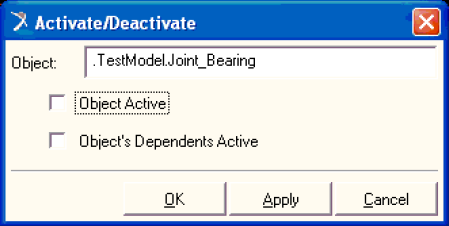
\includegraphics[width=10cm]{figs/JointDeact.png}}
\end{center}
\caption{Joint deactivation dialog \label{figJointDeact}}
\end{figure}

Next step is creating a reference marker on ground that
will give the correct orientation of the bearing.
Use the Command Navigator - marker - create and
specify the orientation so that the $Z$-axis is the
axis of rotation and gravity has negative $X$ direction.
An example is presented in Figure \ref{figTLMRefMarker}.
Write down the ID of the newly created marker.

\begin{figure}[h]
\begin{center}
   {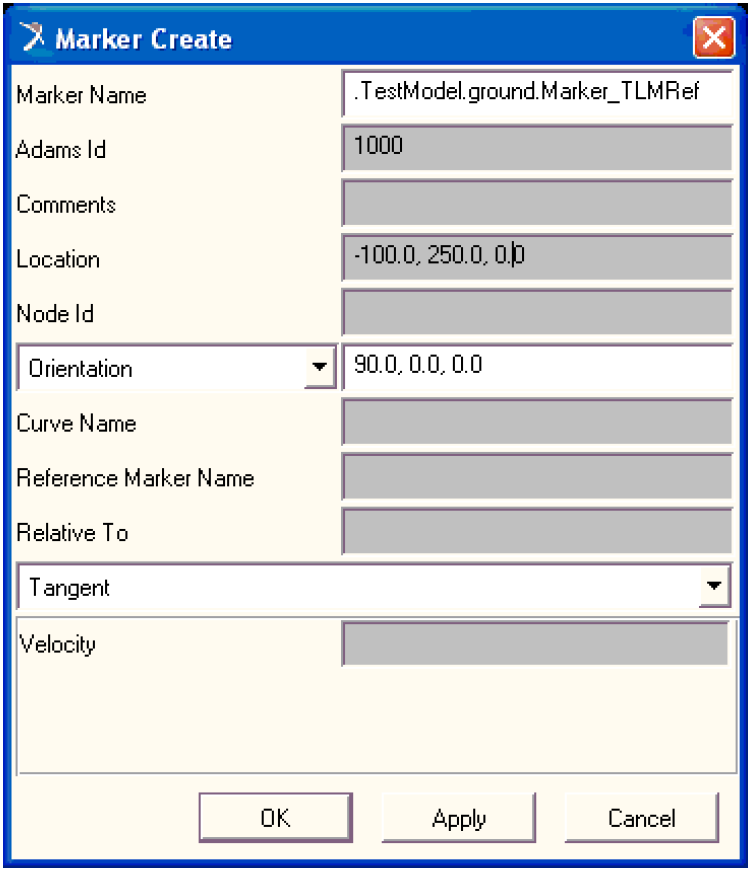
\includegraphics[width=10cm]{figs/TLMRefMarker.png}}
\end{center}
\caption{Create TLM reference marker dialog \label{figTLMRefMarker}}
\end{figure}
Next step is the creation of general forces representing
the TLM connections. Use the Command Navigator-force-
create-direct-general\_force. The Figures \ref{figTLMGFOShaft}
 and \ref{figTLMGFOHousing} presents an example of the dialog.

\begin{figure}[h]
\begin{center}
   {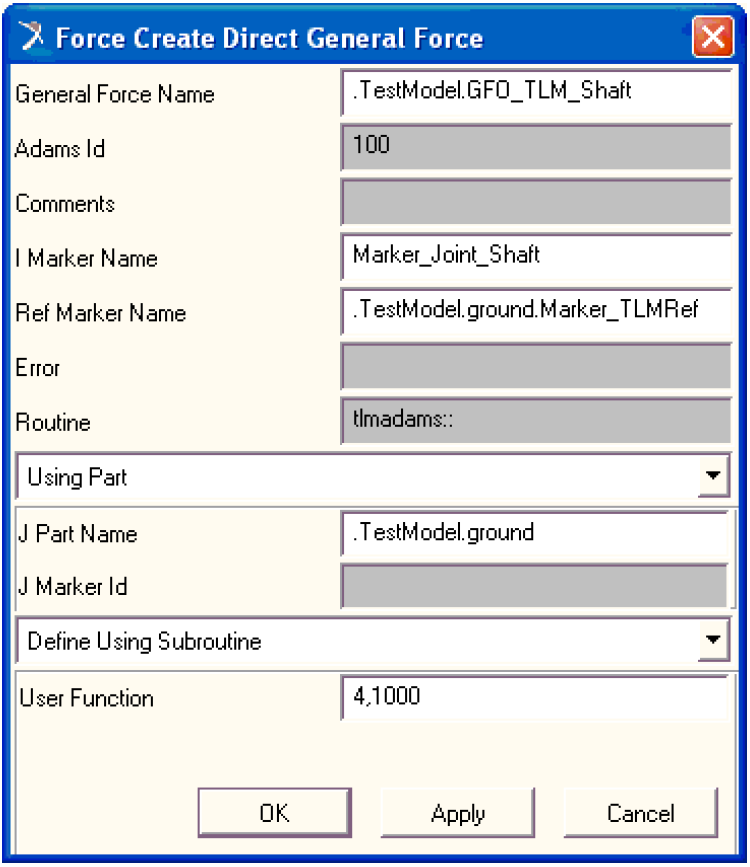
\includegraphics[width=9cm]{figs/TLMGFOShaft.png}}
\end{center}
\caption{Create general force on shaft for TLM dialog \label{figTLMGFOShaft}}
\end{figure}
\begin{figure}
\begin{center}
   {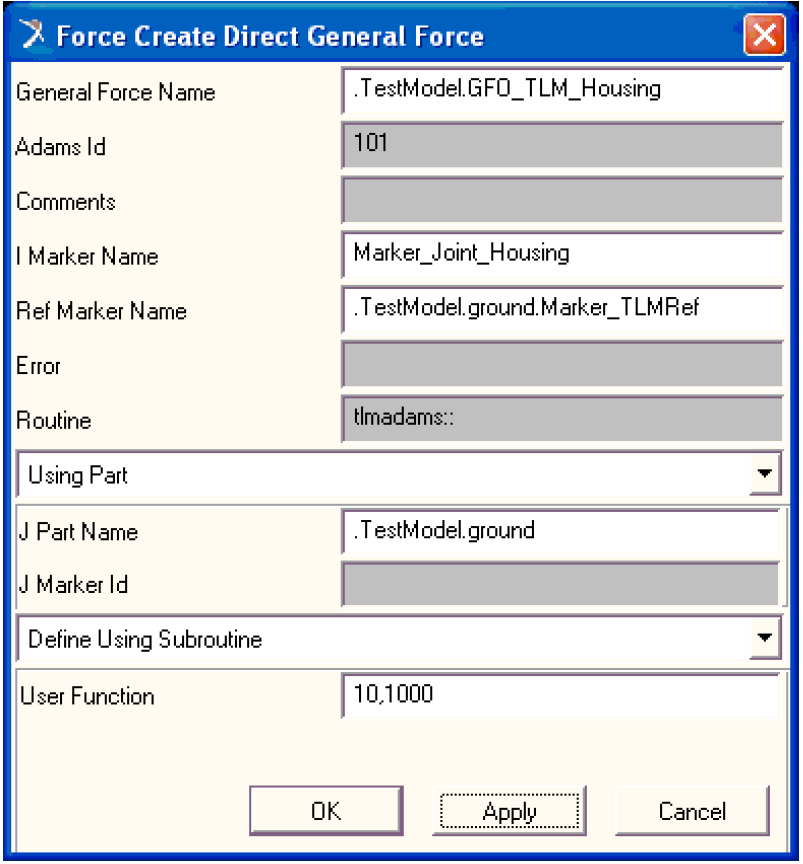
\includegraphics[width=9cm]{figs/TLMGFOHousing.png}}
\end{center}
\caption{Create general force on housing for TLM dialog \label{figTLMGFOHousing}}
\end{figure}

The ADAMS solver dataset can now be exported via the export
dialog as shown in Figure \ref{figADMExport}
\textbf{NOTE} that "Verify the model" check box is off (verification
will result in an unsuccessful call to tlmmanager that crashes the ADAMS/View).

\begin{figure}[h]
\begin{center}
   {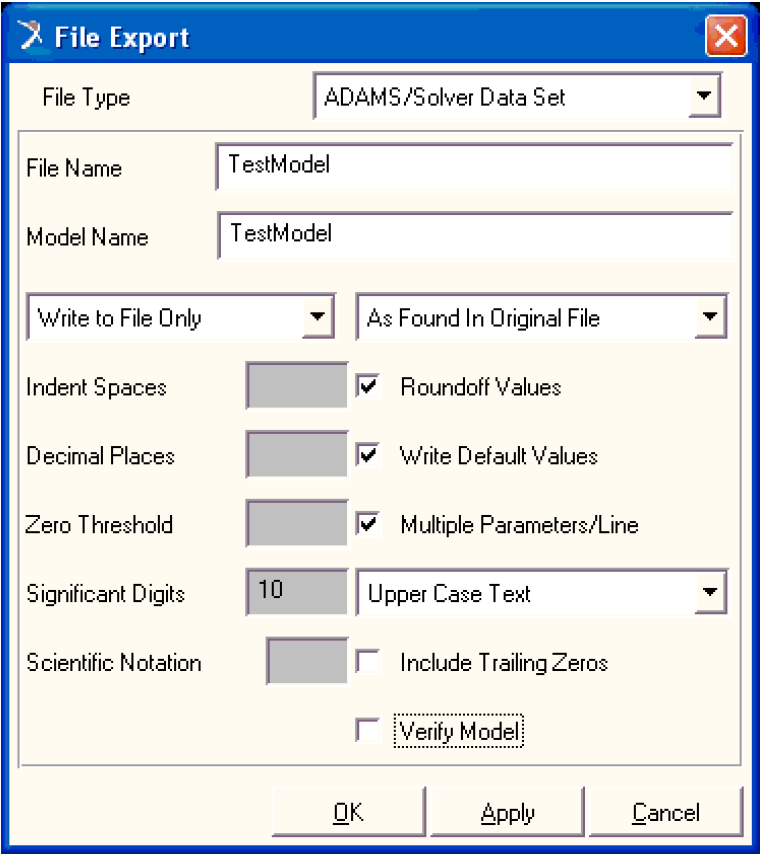
\includegraphics[width=9cm]{figs/TLMExportADM.png}}
\end{center}
\caption{Create general force on housing for TLM dialog \label{figADMExport}}
\end{figure}

TLM co-simulation is sensitive to the consistence of
the velocity initial conditions. The
simulation will start and run even if the initial
velocities are not consistent, however high amplitude
vibrarions in the TLM element with the frequency of
$\omega_{TLM}$ as defined in Equation \ref{eqTspring}
Section \ref{secTLMtheory} will show up in the system.
Therefore it is recommended to
start the simulation with zero velocities in all the
components and simulate a smooth transition to the
working velocities.
\clearpage

\section{Preparing the Scripts}
\label{adams:startup-script}
The next step is creation of an appropriate Adams Command File (.acf).
The file should start a transient simulation of your model.

{\bf Important note:}\\ The current version of the meta-model
simulation environment does not propagate time-settings from the
meta-model to the MSC.ADAMS models automatically. Therfore users need
to check that "time" and "endTime" correspond to the times in the
meta-model.  Check that the integrator parameter Hmax is set to be
less than TLM Delay/2 (use INTEGRATOR command).

An example ACF file is given in Figure \ref{figACFEx}.
\begin{figure}[h]
\small{
\begin{verbatim}
Pendulum
Pendulum_out
INTEGRATOR/SI2, GSTIFF, ERROR=1.0E-6,
HMAX=0.25e-5, HINIT=1.0E-6, LIST
sim/dyn, end=1e-3, steps=10
stop
\end{verbatim}
}
\caption{An example ACF (Adams Command File)\label{figACFEx}}
\end{figure}


A startup script for running the ADAMS simulation needs to be created
as well. A default script is distributed with the BEAST/MME
installation. It is called StartTLMAdams.bat.

{\bf Note:} The default \verb!StartTLMAdams.bat! Windows script needs to
be checked. This should probably be done together with a system
administrator and a member of the BEAST team. However below is a short
discussion of the script for advanced users.

Figure \ref{figStartadams} presents a template for the start script.
The \verb!StartTLMAdams.bat! should first generate a file \verb!tlm.config!
that will contain the parameter send to it by TLM manager.
Only the line giving start command for ADAMS needs to be changed.
For instance, for ADAMS car the line should read:
\begin{verbatim}
set ADAMSSCRIPT=mdi acar ru-so
\end{verbatim}

\begin{figure}[h]
\small{
\begin{verbatim}
@echo off
rem If other parameters are used for ADAMS, change the next line

set ADAMSSCRIPT=mdi ru-s

rem ***************************************************************
rem Changes below should not be necessary

if not a%1==a goto startadams
echo This script is used by TLM manager to start ADAMS simulations
echo It should result in a call to the mdi script
echo for running a simulation according to the specified ACF file
exit 1

:startadams

echo Simulation directory is %1
cd %1

echo Starting an ADAMS simulation with input file: %6.acf
echo Make sure that:
echo time = %2
echo timeEnd = %3
echo MaxTimeStep "<"= %4
echo Writing server configuration to file tlm.config

echo %1 > tlm.config
echo %2 >> tlm.config
echo %3 >> tlm.config
echo %4 >> tlm.config
echo %5 >> tlm.config

echo Starting ADAMS

%ADAMSSCRIPT% %6 > %6.simlog
\end{verbatim}
}
\caption{A template for the \emph{startadams.bat} script\label{figStartadams}}
\end{figure}

Finally, make the \verb!tlmadams.dll! library is accessible for the ADAMS solver.
The simplest way is to copy the library file to your working directory.


